\documentclass[10pt]{beamer}
\usetheme{jambro}

\title[]{Macroeconomia I - Demanda agregada}
\author[]{\href{https://pvfonseca.github.io}{Paulo Victor da Fonseca}}
\date{}

\hypersetup{
    colorlinks = true,
    urlcolor = teal,
    linkcolor = teal    
}
\usepackage[portuguese]{babel}
\usepackage{subfig}
\usepackage{emoji}

\begin{document}

\begin{frame}[plain]
    \titlepage{
        \begin{center}
            \begin{minipage}{0.8\textwidth}
                \centering
            \end{minipage}
        \end{center}}
\end{frame}

\begin{frame}{Sumário}
    \tableofcontents
\end{frame}

\section{Introdução}
\begin{frame}
    {Introdução}
    \begin{itemize}
        \item Na aula anterior vimos o equilíbrio no mercado de bens e serviços em termos da igualdade entre produção e demanda agregada\bigskip
        \item Neste caso, o produto de equilíbrio é igual ao produto entre multiplicador keynesiano e gasto autônomo:
              \[
                  Y = \frac{1}{1-c_1}[c_0 + \bar{I} + G - c_1T]
              \]
        \item Hoje veremos uma forma alternativa (equivalente) de pensarmos o equilíbrio em termos de poupança e investimento\bigskip
        \item Como feito, originalmente, por Keynes na Teoria Geral do Emprego, dos Juros e da Moeda em 1936
    \end{itemize}
\end{frame}

\begin{frame}
    {Poupança privada}
    \begin{itemize}
        \item Examinaremos, inicialmente, o nível de \hlight{poupança} nesta economia: soma das poupanças privada e pública\bigskip
        \item Por definição, a \hlight{poupança privada ($S$)}, poupança dos consumidores, é igual à renda disponível menos consumo:
              \begin{equation}
                  S \equiv Y_D - C
              \end{equation}
        \item Usando a definição de renda disponível, temos:
              \[
                  S \equiv Y - T - C
              \]
    \end{itemize}
\end{frame}

\begin{frame}{Poupança pública}
    \begin{itemize}
        \item Por definição, a \hlight{poupança pública ($S_G$)} é dada pela diferença entre as arrecadações com impostos por parte do governo (líquidos de transferências) e os gastos do governo:
              \begin{equation}
                  S_G \equiv T - G
              \end{equation}

        \item Se os impostos excedem os gastos do governo este governo apresenta um \textbf{superávit orçamentário}, logo, a poupança pública é positiva $S_G>0$\bigskip

        \item Se os impostos são inferiores aos gastos do governo, temos uma situação de \textbf{déficit orçamentário} e a poupança pública é negativa $S_G<0$
    \end{itemize}
\end{frame}

\subsection{Equilíbrio no mercado de bens e serviços}
\begin{frame}{Equilíbrio no mercado de bens: Poupança e investimento}
    \begin{itemize}
        \item Condição de equilíbrio no mercado de bens e serviços: produção deve ser igual à demanda que, por sua vez, é a soma de consumo, investimento e gastos do governo:
              \[
                  Y = C + I + G
              \]

        \item Subtraindo os dois lados da equação pelos impostos $T$ e consumo $C$, temos:
              \[
                  Y - T - C = I + G - T.
              \]

        \item O lado esquerdo da equação é simplesmente a poupança privada $S$, logo:
              \[
                  S = I + G - T,
              \]
              ou, de modo equivalente:
              \begin{eqnarray}
                  I &=& S + (T - G), \nonumber\\
                  I &=& S + S_G. \label{aula5_eq1}
              \end{eqnarray}
    \end{itemize}
\end{frame}

\begin{frame}{Equilíbrio no mercado de bens: Poupança e investimento}
    \begin{itemize}
        \item Equação (\ref{aula5_eq1}): outra forma de pensar equilíbrio no mercado de bens e serviços\bigskip

        \item O equilíbrio no mercado de bens requer que o investimento seja igual à \textbf{poupança} - a soma das poupanças pública e privada\bigskip

        \item Por isso a condição de equilíbrio para o mercado de bens é chamada de \hlight{relação IS} (de \emph{Investment} e \emph{Saving})\bigskip

        \item O que as empresas desejam investir deve ser igual ao que as pessoas e o governo desejam poupar
    \end{itemize}
\end{frame}

\begin{frame}{Equilíbrio no mercado de bens: Poupança e investimento}
    \begin{itemize}
        \item Podemos, então, obter a condição de equilíbrio no mercado de bens usando a condição de que poupança e investimento devem ser consistentes\bigskip

        \item Note que as decisões de consumo e de poupança são iguais. Dada a renda disponível, uma vez que os consumidores tenham escolhido o consumo, sua poupança está determinada, e vice-versa. Portanto, temos:
              \begin{eqnarray}
                  S &=& Y - T - C \nonumber \\
                  S &=& Y - T - c_0 - c_1(Y - T) \nonumber \\
                  S &=& -c_0 + (1 - c_1)(Y - T).
              \end{eqnarray}

        \item Assim como chamamos $c_1$ de propensão marginal a consumir, o termo $(1 - c_1)$ é a \hlight{propensão marginal a poupar} (também entre 0 e 1)\bigskip

        \item Essa propensão nos diz quanto de uma unidade adicional de renda as pessoas estão dispostas a poupar
    \end{itemize}
\end{frame}

\begin{frame}{Equilíbrio no mercado de bens: Poupança e investimento}
    \begin{itemize}
        \item No equilíbrio, investimento deve ser igual à poupança:
              \begin{eqnarray}
                  I &=& S + S_G \nonumber \\
                  I &=& -c_0 + (1 - c_1)(Y - T) + (T - G). \nonumber
              \end{eqnarray}

        \item Resolvendo para o produto agregado de equilíbrio, temos:
              \begin{equation}
                  Y = \frac{1}{1-c_1}[c_0 + \bar{I} + G - c_1T],
                  \label{aula5_eq2}
              \end{equation}
              que é exatamente a mesma equação que derivamos analisando a condição de que produção e demanda são iguais
    \end{itemize}
\end{frame}

\section{Paradoxo da poupança}
\begin{frame}{Paradoxo da poupança}
    \begin{itemize}
        \item Imagine que a economia encontra-se em um período de recessão e o seguinte questionamento é levantado:\bigskip

              \NB{\emoji{question} Devemos adotar uma política macroeconômica de estímulo ou de desincentivo à poupança de forma a assegurar uma recuperação econômica?}\bigskip

        \item Por um lado, um estímulo ao nível de poupança parece desejável: se os agentes econômicos poupam mais e essa poupança é investida em estoque de capital, podemos ter uma receita para a recuperação econômica\bigskip

        \item No entanto, um aumento da poupança significa uma contração no nível de consumo e, caso não haja um aumento no nível de investimento, isso não levaria a uma redução de demanda agregada e, consequentemente, um agravamento da recessão?
    \end{itemize}
\end{frame}

\begin{frame}{Paradoxo da poupança}
    \begin{itemize}
        \item Para respondermos a essa pergunta, devemos investigar como os agentes se comportam no nosso modelo macroeconômico\bigskip

        \item Em um modelo econômico, as hipóteses feitas acerca do comportamento dos agentes são resumidas em \textcolor{purple}{equações comportamentais}\bigskip

        \item No modelo básico que formulamos até agora, a equação comportamental para o consumo agregado é dada pela função de consumo Keynesiana\bigskip

        \item Gastos públicos e investimento privado são, por hipótese, mantidos constantes (variáveis exógenas)
    \end{itemize}
\end{frame}

\begin{frame}{Paradoxo da poupança}
    \begin{itemize}
        \item Vimos, anteriormente, que a soma das poupanças pública e privada é igual ao nível de investimento planejado:
              \[
                  S + S_G = \bar{I}.
              \]

        \item Portanto:
              \[
                  -c_0 + (1-c_1)(Y-T) = \bar{I} - (T-G).
              \]

        \item Modelaremos a proposta de estímulo à poupança privada como uma queda no componente autônomo de consumo de $c_0$ para $c_0'$\bigskip

        \item A demanda agregada, inicialmente, é contraída em uma magnitude $(c_0-c_0')$ e o processo multiplicador opera em uma direção negativa
    \end{itemize}
\end{frame}

\begin{frame}{Paradoxo da poupança}
    \begin{itemize}
        \item Usando o diagrama da cruz Keynesiana, observamos que este processo continua até que um novo equilíbrio seja alcançado a um nível de renda agregada mais baixo\bigskip

        \item Ao novo nível de produto mais baixo, $Y'$, a poupança privada planejada do lado esquerdo da equação é igual ao investimento planejado subtraído da poupança pública, variáveis que não foram alteradas:
              \[
                  -c_0' + (1-c_1)(Y'-T) = \bar{I} - (T-G).
              \]
    \end{itemize}
\end{frame}

\begin{frame}{Paradoxo da poupança}
    \begin{itemize}
        \item Portanto, um \emph{insight} importante emerge deste exemplo\bigskip

        \item O equilíbrio inicial foi perturbado por uma queda no consumo autônomo, à medida que as famílias desejavam aumentar seus níveis de poupança\bigskip

        \item No entanto, a intenção de poupar mais não levou a um aumento no nível agregado de poupança pois a renda agregada diminuiu $\left(\Delta Y = \frac{1}{1-c_1}(c_0-c_0'\right)$\bigskip

              \NB{\hlight{Paradoxo da poupança}: se um nível mais alto de poupança por parte das famílias não for acompanhado por um investimento mais elevado em capital fixo, a renda agregada reduzirá e, portanto, não haverá um aumento na poupança agregada da economia}
    \end{itemize}
\end{frame}

\begin{frame}{Paradoxo da poupança}
    \begin{itemize}
        \item Em resumo, a resposta à questão inicial se devemos estimular um aumento da poupança durante uma recessão depende, fundamentalmente, do modelo econômico que o economista está utilizando e, obviamente, do quão bem este modelo se ajusta aos dados reais da economia considerada\bigskip

        \item No modelo que formulamos até agora a resposta é clara: um estímulo à poupança privada não ajudará a economia a se recuperar de um período de recessão\bigskip

        \item O motivo para isso é que não existe algum mecanismo neste modelo pelo qual um nível mais elevado de poupança se traduza em um investimento mais alto - investimento se mantém fixo em $\bar{I}$\bigskip

        \item Portanto, \hlight{uma maior propensão a poupar implica em uma contração de demanda agregada, uma queda no produto e, consequentemente, um agravamento da recessão}
    \end{itemize}
\end{frame}

\begin{frame}{Paradoxo da poupança}
    \begin{itemize}
        \item Este resultado seria o mesmo se considerássemos a poupança pública: a redução do déficit orçamentário também levaria a uma redução do produto e uma poupança (pública e privada) inalterada\bigskip

        \item O resultado seria ainda mais dramático se permitirmos que o investimento baixe de acordo com o produto: uma tentativa de poupar mais levaria a um produto menor, um investimento menor e, consequentemente, uma poupança menor\bigskip

        \item Por outro lado, se incluirmos uma autoridade monetária ao nosso modelo, a recessão poderia ser evitada com o BC reduzindo a taxa de juros e, então, estimulando o investimento de forma a mitigar a queda na poupança\bigskip
        \item Cabe ressaltar que os resultados deste modelo simples são relevantes no curto prazo. No médio e longo prazos, outros mecanismos entram em jogo ao longo do tempo, e um aumento da taxa de poupança leva, no decorrer do tempo, a uma poupança e renda mais elevadas
    \end{itemize}
\end{frame}

\begin{frame}{Paradoxo da poupança}
    \begin{itemize}
        \item Os aumentos nos níveis de poupança que seguiram a CFG de 2008-2009 e a pandemia recente reacenderam o interesse de economistas e formuladores de política econômica no paradoxo da poupança, formulado por Keynes na década de 1930\bigskip

        \item Como vimos, o paradoxo da poupança afirma que um aumento na poupança não leva, naturalmente, a um aumento no nível de investimentos\bigskip

        \item Pelo contrário, a \hlight{poupança precaucionária} (\emph{precautionary savings}) - poupança adicional resultante de um futuro incerto - é prejudicial ao crescimento econômico dado que \emph{desloca} (\emph{crowds out}) o consumo e, portanto, diminui a demanda agregada
    \end{itemize}
\end{frame}

\begin{frame}{Paradoxo da poupança}
    \begin{itemize}
        \item A pandemia do COVID-19 causou um aumento sem precedentes nos níveis de poupança\bigskip

        \item Na UE, a taxa de poupança das famílias aumentou de 12,5\% para 17\%\bigskip

        \item Durante a CFG de 2008, o aumento foi de 12,5\% para 14\%\bigskip

        \item Mesmo que os motivos sejam diferentes agora, é óbvio que este aumento nos níveis de poupança não resulta em um aumento dos investimentos e do crescimento econômico\bigskip

        \item Dadas as expectativas pessimistas e incertezas nos mercados de trabalho e de créditos, é mais provável que essa poupança forçada acumulada durante as medidas de restrição será parcialmente transformada em poupança precaucionária
    \end{itemize}
\end{frame}

\begin{frame}{Paradoxo da poupança}
    \begin{itemize}
        \item Por estas razões, os formuladores de política econômica encorajaram fortemente o consumo assim que as condições sanitárias permitiram\bigskip

        \item Estas situações são similares àquelas enfrentadas por Keynes em 1931:\bigskip
              \NB{
                  There are today many well-wishers of their country who believe that the most useful thing which they and their neighbours can do to mend the situation is to save more than usual. […] It is utterly harmful and misguided – the very opposite of the truth.
                  \begin{flushright}
                      (Keynes, 1931 - Essays in Persuasion).
                  \end{flushright}}
    \end{itemize}
\end{frame}

\begin{frame}{Paradoxo da poupança}
    \begin{itemize}
        \item A proporção dos depósitos de poupança com relação ao PIB aumentou mais naqueles países onde o PIB real apresentou um crescimento menor
    \end{itemize}
    \begin{figure}
        \centering
        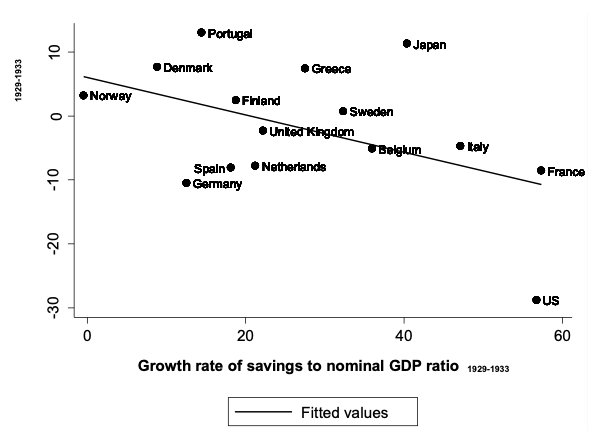
\includegraphics[width=0.5\textwidth]{./figures/aula6_fig1.jpg}
        \caption{Correlação entre o aumento na taxa de poupança e crescimento do PIB real durante a Grande Depressão, 1929-1933. Fonte: Degorce e Monnet (2020).}
        \label{aula5_fig1}
    \end{figure}
\end{frame}

\section{Exercícios}
\begin{frame}{Exercícios}
    Suponha que a economia seja caracterizada pelas seguintes equações comportamentais:
    \begin{eqnarray}
        C &=& 160 + 0,6Y_D, \nonumber \\
        I &=& 150, \nonumber \\
        G &=& 150, \nonumber \\
        T &=& 100. \nonumber
    \end{eqnarray}
    Resolva para as seguintes variáveis:
    \begin{enumerate}
        \item O PIB de equilíbrio ($Y$).

        \item A renda disponível ($Y_D$).

        \item Os gastos de consumo ($C$).

        \item Poupanças pública e privada de equilíbrio.
    \end{enumerate}
\end{frame}

\begin{frame}{Exercícios}
    Considere uma economia representada pelas seguintes equações:
    \begin{eqnarray}
        C &=& 400 + 0,5Y_D, \nonumber \\
        I &=& 300, \nonumber \\
        T &=& 100 + 0,2Y, \nonumber \\
        G &=& 250. \nonumber
    \end{eqnarray}
    \begin{enumerate}
        \item Produto de equilíbrio.

        \item Impostos de equilíbrio.

        \item Poupanças pública e privada de equilíbrio.

        \item Se a alíquota de imposto for reduzida para a zero, tudo o mais constante, qual a expansão do produto?
    \end{enumerate}
\end{frame}

\section{Papel da política fiscal}
\begin{frame}{Política fiscal}
    \begin{itemize}
        \item A equação (\ref{aula5_eq2}) implica que a decisão de política fiscal por parte do governo - escolha do nível de gastos públicos ($G$) ou dos impostos ($T$) - pode ser feita de maneira a atingir um nível de produto agregado desejado\bigskip

        \item É esse realmente o caso? Os governos podem escolher o nível de produto que quiserem?\bigskip

        \item Ainda existem muitos aspectos da realidade que não foram incorporados ao modelo, e todos eles complicam a tarefa do governo
    \end{itemize}
\end{frame}

\begin{frame}{Política fiscal}
    \begin{enumerate}
        \item Uma mudança de gastos do governo ou do nível de impostos pode ser difícil\bigskip

        \item Até agora assumimos que o nível de investimentos é constante e exogenamente determinado. Fizemos o mesmo para importações, mas parte do aumento da demanda pode ser por bens importados. Todas essas respostas estão associadas a efeitos dinâmicos complexos, dificultando a avaliação precisa por parte do governo\bigskip

        \item Expectativas são importantes. Exemplo: a reação dos consumidores a corte nos impostos depende de como eles percebem - transitório ou permanente. Quanto maior a percepção de que o corte é permanente, maior será a resposta do consumo. De modo análogo, a reação dos consumidores a aumento nos gastos públicos deve depender de quando os agentes acham que o governo elevará impostos para cobrir os gastos

    \end{enumerate}
\end{frame}

\begin{frame}{Política fiscal}
    \begin{enumerate}

        \item[4] Atingir um dado nível de produto pode estar associado a efeitos adversos. Exemplo: a tentativa de alcançar um nível muito elevado de produto agregado pode levar a uma inflação crescente e, por este motivo, tornar-se insustentável no médio prazo\bigskip

        \item[5] O corte de impostos ou aumento dos gastos públicos podem levar a grandes déficits orçamentários e a um aumento do estoque de dívida pública. Uma dívida elevada pode ter efeitos adversos no longo prazo
    \end{enumerate}
\end{frame}

\begin{frame}{Política fiscal}
    \begin{itemize}
        \item Em resumo, a proposição de que o governo pode afetar a demanda e o produto no curto prazo via política fiscal é correta e importante\bigskip

        \item Mas, à medida que refinarmos nosso modelo, veremos que o papel do governo, de modo geral e, principalmente, o uso bem sucedido da política fiscal se tornarão cada vez mais difíceis
    \end{itemize}
\end{frame}

\begin{frame}{\emoji{books} Bibliografia}
    \begin{itemize}
        \item BLANCHARD, O. Macroeconomia. 7.ed. São Paulo: Pearson Education do Brasil, 2017\medskip
        \item DEGORCE, V; MONNET, E. \href{https://papers.ssrn.com/sol3/papers.cfm?abstract_id=3696369}{The Great Depression as a Saving Glut}, CEPR Discussion Papers 15287, 2020\medskip
              %\item CARLIN, W.; SOSKICE, D. Macroeconomics: Institutions, instability, and the financial system. Oxford, UK: Oxford University Press, 2015\medskip
              %\item DORNBUSCH, R.; FISCHER, S.; STARTZ, R. Macroeconomia. 11.ed. Porto Alegre: AMGH, 2013. Disponível em: \href{https://app.minhabiblioteca.com.br/books/9788580551853}{app.minhabiblioteca.com.br/books/9788580551853}\medskip
        \item KEYNES, J.M. \emph{A teoria geral do emprego, do juro e da moeda}. São Paulo: Atlas, 1992. (Data do original em inglês: 1936)\medskip
    \end{itemize}
\end{frame}
\end{document}